% Created by tikzDevice version 0.10.1 on 2016-08-19 17:06:53
% !TEX encoding = UTF-8 Unicode
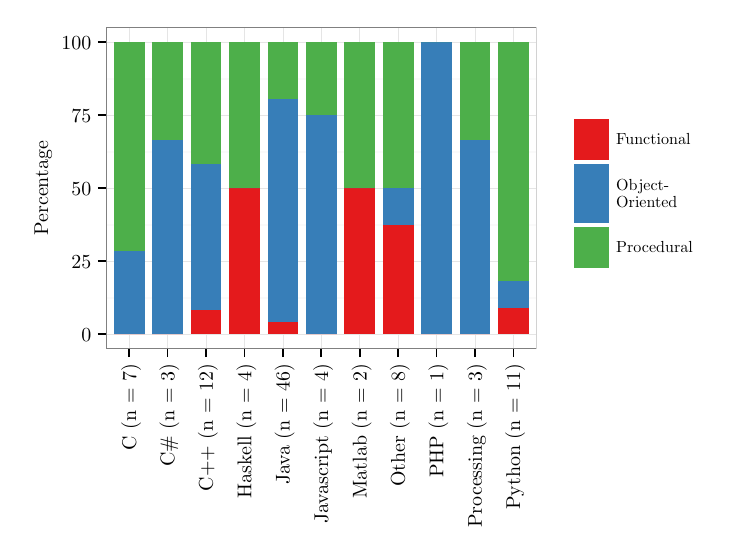
\begin{tikzpicture}[x=1pt,y=1pt]
\definecolor{fillColor}{RGB}{255,255,255}
\path[use as bounding box,fill=fillColor,fill opacity=0.00] (0,0) rectangle (252.94,180.67);
\begin{scope}
\path[clip] (  0.00,  0.00) rectangle (252.94,180.67);
\definecolor{drawColor}{RGB}{255,255,255}
\definecolor{fillColor}{RGB}{255,255,255}

\path[draw=drawColor,line width= 0.6pt,line join=round,line cap=round,fill=fillColor] (  0.00,  0.00) rectangle (252.94,180.68);
\end{scope}
\begin{scope}
\path[clip] ( 28.36, 64.59) rectangle (183.84,180.67);
\definecolor{fillColor}{RGB}{255,255,255}

\path[fill=fillColor] ( 28.36, 64.59) rectangle (183.84,180.68);
\definecolor{drawColor}{gray}{0.98}

\path[draw=drawColor,line width= 0.6pt,line join=round] ( 28.36, 83.05) --
	(183.84, 83.05);

\path[draw=drawColor,line width= 0.6pt,line join=round] ( 28.36,109.44) --
	(183.84,109.44);

\path[draw=drawColor,line width= 0.6pt,line join=round] ( 28.36,135.82) --
	(183.84,135.82);

\path[draw=drawColor,line width= 0.6pt,line join=round] ( 28.36,162.21) --
	(183.84,162.21);
\definecolor{drawColor}{gray}{0.90}

\path[draw=drawColor,line width= 0.2pt,line join=round] ( 28.36, 69.86) --
	(183.84, 69.86);

\path[draw=drawColor,line width= 0.2pt,line join=round] ( 28.36, 96.25) --
	(183.84, 96.25);

\path[draw=drawColor,line width= 0.2pt,line join=round] ( 28.36,122.63) --
	(183.84,122.63);

\path[draw=drawColor,line width= 0.2pt,line join=round] ( 28.36,149.01) --
	(183.84,149.01);

\path[draw=drawColor,line width= 0.2pt,line join=round] ( 28.36,175.40) --
	(183.84,175.40);

\path[draw=drawColor,line width= 0.2pt,line join=round] ( 36.69, 64.59) --
	( 36.69,180.67);

\path[draw=drawColor,line width= 0.2pt,line join=round] ( 50.57, 64.59) --
	( 50.57,180.67);

\path[draw=drawColor,line width= 0.2pt,line join=round] ( 64.45, 64.59) --
	( 64.45,180.67);

\path[draw=drawColor,line width= 0.2pt,line join=round] ( 78.33, 64.59) --
	( 78.33,180.67);

\path[draw=drawColor,line width= 0.2pt,line join=round] ( 92.22, 64.59) --
	( 92.22,180.67);

\path[draw=drawColor,line width= 0.2pt,line join=round] (106.10, 64.59) --
	(106.10,180.67);

\path[draw=drawColor,line width= 0.2pt,line join=round] (119.98, 64.59) --
	(119.98,180.67);

\path[draw=drawColor,line width= 0.2pt,line join=round] (133.86, 64.59) --
	(133.86,180.67);

\path[draw=drawColor,line width= 0.2pt,line join=round] (147.74, 64.59) --
	(147.74,180.67);

\path[draw=drawColor,line width= 0.2pt,line join=round] (161.63, 64.59) --
	(161.63,180.67);

\path[draw=drawColor,line width= 0.2pt,line join=round] (175.51, 64.59) --
	(175.51,180.67);
\definecolor{fillColor}{RGB}{228,26,28}

\path[fill=fillColor] ( 31.13, 69.86) rectangle ( 42.24, 69.86);
\definecolor{fillColor}{RGB}{55,126,184}

\path[fill=fillColor] ( 31.13, 69.86) rectangle ( 42.24,100.02);
\definecolor{fillColor}{RGB}{77,175,74}

\path[fill=fillColor] ( 31.13,100.02) rectangle ( 42.24,175.40);
\definecolor{fillColor}{RGB}{228,26,28}

\path[fill=fillColor] ( 45.02, 69.86) rectangle ( 56.12, 69.86);
\definecolor{fillColor}{RGB}{55,126,184}

\path[fill=fillColor] ( 45.02, 69.86) rectangle ( 56.12,140.22);
\definecolor{fillColor}{RGB}{77,175,74}

\path[fill=fillColor] ( 45.02,140.22) rectangle ( 56.12,175.40);
\definecolor{fillColor}{RGB}{228,26,28}

\path[fill=fillColor] ( 58.90, 69.86) rectangle ( 70.00, 78.66);
\definecolor{fillColor}{RGB}{55,126,184}

\path[fill=fillColor] ( 58.90, 78.66) rectangle ( 70.00,131.42);
\definecolor{fillColor}{RGB}{77,175,74}

\path[fill=fillColor] ( 58.90,131.42) rectangle ( 70.00,175.40);
\definecolor{fillColor}{RGB}{228,26,28}

\path[fill=fillColor] ( 72.78, 69.86) rectangle ( 83.89,122.63);
\definecolor{fillColor}{RGB}{55,126,184}

\path[fill=fillColor] ( 72.78,122.63) rectangle ( 83.89,122.63);
\definecolor{fillColor}{RGB}{77,175,74}

\path[fill=fillColor] ( 72.78,122.63) rectangle ( 83.89,175.40);
\definecolor{fillColor}{RGB}{228,26,28}

\path[fill=fillColor] ( 86.66, 69.86) rectangle ( 97.77, 74.45);
\definecolor{fillColor}{RGB}{55,126,184}

\path[fill=fillColor] ( 86.66, 74.45) rectangle ( 97.77,154.75);
\definecolor{fillColor}{RGB}{77,175,74}

\path[fill=fillColor] ( 86.66,154.75) rectangle ( 97.77,175.40);
\definecolor{fillColor}{RGB}{228,26,28}

\path[fill=fillColor] (100.54, 69.86) rectangle (111.65, 69.86);
\definecolor{fillColor}{RGB}{55,126,184}

\path[fill=fillColor] (100.54, 69.86) rectangle (111.65,149.01);
\definecolor{fillColor}{RGB}{77,175,74}

\path[fill=fillColor] (100.54,149.01) rectangle (111.65,175.40);
\definecolor{fillColor}{RGB}{228,26,28}

\path[fill=fillColor] (114.43, 69.86) rectangle (125.53,122.63);
\definecolor{fillColor}{RGB}{55,126,184}

\path[fill=fillColor] (114.43,122.63) rectangle (125.53,122.63);
\definecolor{fillColor}{RGB}{77,175,74}

\path[fill=fillColor] (114.43,122.63) rectangle (125.53,175.40);
\definecolor{fillColor}{RGB}{228,26,28}

\path[fill=fillColor] (128.31, 69.86) rectangle (139.42,109.44);
\definecolor{fillColor}{RGB}{55,126,184}

\path[fill=fillColor] (128.31,109.44) rectangle (139.42,122.63);
\definecolor{fillColor}{RGB}{77,175,74}

\path[fill=fillColor] (128.31,122.63) rectangle (139.42,175.40);
\definecolor{fillColor}{RGB}{228,26,28}

\path[fill=fillColor] (142.19, 69.86) rectangle (153.30, 69.86);
\definecolor{fillColor}{RGB}{55,126,184}

\path[fill=fillColor] (142.19, 69.86) rectangle (153.30,175.40);
\definecolor{fillColor}{RGB}{77,175,74}

\path[fill=fillColor] (142.19,175.40) rectangle (153.30,175.40);
\definecolor{fillColor}{RGB}{228,26,28}

\path[fill=fillColor] (156.07, 69.86) rectangle (167.18, 69.86);
\definecolor{fillColor}{RGB}{55,126,184}

\path[fill=fillColor] (156.07, 69.86) rectangle (167.18,140.22);
\definecolor{fillColor}{RGB}{77,175,74}

\path[fill=fillColor] (156.07,140.22) rectangle (167.18,175.40);
\definecolor{fillColor}{RGB}{228,26,28}

\path[fill=fillColor] (169.96, 69.86) rectangle (181.06, 79.46);
\definecolor{fillColor}{RGB}{55,126,184}

\path[fill=fillColor] (169.96, 79.46) rectangle (181.06, 89.05);
\definecolor{fillColor}{RGB}{77,175,74}

\path[fill=fillColor] (169.96, 89.05) rectangle (181.06,175.40);
\definecolor{drawColor}{gray}{0.50}

\path[draw=drawColor,line width= 0.6pt,line join=round,line cap=round] ( 28.36, 64.59) rectangle (183.84,180.68);
\end{scope}
\begin{scope}
\path[clip] (  0.00,  0.00) rectangle (252.94,180.67);
\definecolor{drawColor}{RGB}{0,0,0}

\node[text=drawColor,anchor=base east,inner sep=0pt, outer sep=0pt, scale=  0.72] at ( 22.96, 67.38) {0};

\node[text=drawColor,anchor=base east,inner sep=0pt, outer sep=0pt, scale=  0.72] at ( 22.96, 93.77) {25};

\node[text=drawColor,anchor=base east,inner sep=0pt, outer sep=0pt, scale=  0.72] at ( 22.96,120.15) {50};

\node[text=drawColor,anchor=base east,inner sep=0pt, outer sep=0pt, scale=  0.72] at ( 22.96,146.53) {75};

\node[text=drawColor,anchor=base east,inner sep=0pt, outer sep=0pt, scale=  0.72] at ( 22.96,172.92) {100};
\end{scope}
\begin{scope}
\path[clip] (  0.00,  0.00) rectangle (252.94,180.67);
\definecolor{drawColor}{RGB}{0,0,0}

\path[draw=drawColor,line width= 0.6pt,line join=round] ( 25.36, 69.86) --
	( 28.36, 69.86);

\path[draw=drawColor,line width= 0.6pt,line join=round] ( 25.36, 96.25) --
	( 28.36, 96.25);

\path[draw=drawColor,line width= 0.6pt,line join=round] ( 25.36,122.63) --
	( 28.36,122.63);

\path[draw=drawColor,line width= 0.6pt,line join=round] ( 25.36,149.01) --
	( 28.36,149.01);

\path[draw=drawColor,line width= 0.6pt,line join=round] ( 25.36,175.40) --
	( 28.36,175.40);
\end{scope}
\begin{scope}
\path[clip] (  0.00,  0.00) rectangle (252.94,180.67);
\definecolor{drawColor}{RGB}{0,0,0}

\path[draw=drawColor,line width= 0.6pt,line join=round] ( 36.69, 61.59) --
	( 36.69, 64.59);

\path[draw=drawColor,line width= 0.6pt,line join=round] ( 50.57, 61.59) --
	( 50.57, 64.59);

\path[draw=drawColor,line width= 0.6pt,line join=round] ( 64.45, 61.59) --
	( 64.45, 64.59);

\path[draw=drawColor,line width= 0.6pt,line join=round] ( 78.33, 61.59) --
	( 78.33, 64.59);

\path[draw=drawColor,line width= 0.6pt,line join=round] ( 92.22, 61.59) --
	( 92.22, 64.59);

\path[draw=drawColor,line width= 0.6pt,line join=round] (106.10, 61.59) --
	(106.10, 64.59);

\path[draw=drawColor,line width= 0.6pt,line join=round] (119.98, 61.59) --
	(119.98, 64.59);

\path[draw=drawColor,line width= 0.6pt,line join=round] (133.86, 61.59) --
	(133.86, 64.59);

\path[draw=drawColor,line width= 0.6pt,line join=round] (147.74, 61.59) --
	(147.74, 64.59);

\path[draw=drawColor,line width= 0.6pt,line join=round] (161.63, 61.59) --
	(161.63, 64.59);

\path[draw=drawColor,line width= 0.6pt,line join=round] (175.51, 61.59) --
	(175.51, 64.59);
\end{scope}
\begin{scope}
\path[clip] (  0.00,  0.00) rectangle (252.94,180.67);
\definecolor{drawColor}{RGB}{0,0,0}

\node[text=drawColor,rotate= 90.00,anchor=base east,inner sep=0pt, outer sep=0pt, scale=  0.72] at ( 39.16, 59.19) {C (n = 7)};

\node[text=drawColor,rotate= 90.00,anchor=base east,inner sep=0pt, outer sep=0pt, scale=  0.72] at ( 53.05, 59.19) {C\# (n = 3)};

\node[text=drawColor,rotate= 90.00,anchor=base east,inner sep=0pt, outer sep=0pt, scale=  0.72] at ( 66.93, 59.19) {C++ (n = 12)};

\node[text=drawColor,rotate= 90.00,anchor=base east,inner sep=0pt, outer sep=0pt, scale=  0.72] at ( 80.81, 59.19) {Haskell (n = 4)};

\node[text=drawColor,rotate= 90.00,anchor=base east,inner sep=0pt, outer sep=0pt, scale=  0.72] at ( 94.69, 59.19) {Java (n = 46)};

\node[text=drawColor,rotate= 90.00,anchor=base east,inner sep=0pt, outer sep=0pt, scale=  0.72] at (108.58, 59.19) {Javascript (n = 4)};

\node[text=drawColor,rotate= 90.00,anchor=base east,inner sep=0pt, outer sep=0pt, scale=  0.72] at (122.46, 59.19) {Matlab (n = 2)};

\node[text=drawColor,rotate= 90.00,anchor=base east,inner sep=0pt, outer sep=0pt, scale=  0.72] at (136.34, 59.19) {Other (n = 8)};

\node[text=drawColor,rotate= 90.00,anchor=base east,inner sep=0pt, outer sep=0pt, scale=  0.72] at (150.22, 59.19) {PHP (n = 1)};

\node[text=drawColor,rotate= 90.00,anchor=base east,inner sep=0pt, outer sep=0pt, scale=  0.72] at (164.11, 59.19) {Processing (n = 3)};

\node[text=drawColor,rotate= 90.00,anchor=base east,inner sep=0pt, outer sep=0pt, scale=  0.72] at (177.99, 59.19) {Python (n = 11)};
\end{scope}
\begin{scope}
\path[clip] (  0.00,  0.00) rectangle (252.94,180.67);
\definecolor{drawColor}{RGB}{0,0,0}

\node[text=drawColor,rotate= 90.00,anchor=base,inner sep=0pt, outer sep=0pt, scale=  0.72] at (  7.36,122.63) {Percentage};
\end{scope}
\begin{scope}
\path[clip] (  0.00,  0.00) rectangle (252.94,180.67);
\definecolor{fillColor}{RGB}{255,255,255}

\path[fill=fillColor] (192.37, 88.83) rectangle (244.41,156.43);
\end{scope}
\begin{scope}
\path[clip] (  0.00,  0.00) rectangle (252.94,180.67);
\definecolor{fillColor}{RGB}{228,26,28}

\path[fill=fillColor] (197.35,132.85) rectangle (210.16,147.84);
\end{scope}
\begin{scope}
\path[clip] (  0.00,  0.00) rectangle (252.94,180.67);
\definecolor{fillColor}{RGB}{55,126,184}

\path[fill=fillColor] (197.35,110.22) rectangle (210.16,131.43);
\end{scope}
\begin{scope}
\path[clip] (  0.00,  0.00) rectangle (252.94,180.67);
\definecolor{fillColor}{RGB}{77,175,74}

\path[fill=fillColor] (197.35, 93.81) rectangle (210.16,108.80);
\end{scope}
\begin{scope}
\path[clip] (  0.00,  0.00) rectangle (252.94,180.67);
\definecolor{drawColor}{RGB}{0,0,0}

\node[text=drawColor,anchor=base west,inner sep=0pt, outer sep=0pt, scale=  0.58] at (212.68,144.58) {};

\node[text=drawColor,anchor=base west,inner sep=0pt, outer sep=0pt, scale=  0.58] at (212.68,138.36) {Functional};

\node[text=drawColor,anchor=base west,inner sep=0pt, outer sep=0pt, scale=  0.58] at (212.68,132.14) {};
\end{scope}
\begin{scope}
\path[clip] (  0.00,  0.00) rectangle (252.94,180.67);
\definecolor{drawColor}{RGB}{0,0,0}

\node[text=drawColor,anchor=base west,inner sep=0pt, outer sep=0pt, scale=  0.58] at (212.68,128.17) {};

\node[text=drawColor,anchor=base west,inner sep=0pt, outer sep=0pt, scale=  0.58] at (212.68,121.95) {Object-};

\node[text=drawColor,anchor=base west,inner sep=0pt, outer sep=0pt, scale=  0.58] at (212.68,115.73) {Oriented};

\node[text=drawColor,anchor=base west,inner sep=0pt, outer sep=0pt, scale=  0.58] at (212.68,109.51) {};
\end{scope}
\begin{scope}
\path[clip] (  0.00,  0.00) rectangle (252.94,180.67);
\definecolor{drawColor}{RGB}{0,0,0}

\node[text=drawColor,anchor=base west,inner sep=0pt, outer sep=0pt, scale=  0.58] at (212.68,105.54) {};

\node[text=drawColor,anchor=base west,inner sep=0pt, outer sep=0pt, scale=  0.58] at (212.68, 99.32) {Procedural};

\node[text=drawColor,anchor=base west,inner sep=0pt, outer sep=0pt, scale=  0.58] at (212.68, 93.10) {};
\end{scope}
\end{tikzpicture}
